\documentclass[11pt]{report}

\usepackage{helvet}
\renewcommand{\familydefault}{\sfdefault}
\renewcommand{\rmdefault}{\sfdefault}
%\usepackage{sfmath}
%\usepackage{sansmath}

\usepackage[utf8]{inputenc}
\usepackage[czech]{babel}
\usepackage{amsfonts,amsmath}
\usepackage{etoolbox}
\usepackage{graphicx}
% \usepackage{hyperref}
\usepackage{multirow}
\usepackage{titlesec}
\setcounter{secnumdepth}{3}
\usepackage[total={8.27in, 11.60in}, left=0.82in, right=0.82in,%
top=1.49in, bottom=1.49in]{geometry}
\usepackage{float}
\usepackage{caption}
\usepackage{subcaption}

\usepackage{fancyhdr}
\pagestyle{fancy}
\lhead{
    \begin{picture}(0,0)
        \put(-60,0){
\includegraphics{TACR_logo.png}}
    \end{picture}
    }
\rhead{}    
\cfoot{}
\rfoot{\thepage}
\renewcommand{\headrulewidth}{0pt}

\usepackage{tikz}

% macro for units.
\def\UNIT#1#2{\ifstrempty{#2}{}{%
\ifstrequal{#2}{1}{\mathrm{#1}}{\mathrm{#1}^{#2}}%
}}
\def\units#1#2#3{\ifstrempty{#1#2#3}{$[-]$}{$[ \UNIT{kg}{#1}\UNIT{m}{#2}\UNIT{s}{#3} ]$}} %with brackets
\def\unitss#1#2#3{\ifstrempty{#1#2#3}{$-$}{$ \UNIT{kg}{#1}\UNIT{m}{#2}\UNIT{s}{#3} $}}    %without brackets

%macro for hyperlinks (dummy)
\def\hyperA#1#2{#2}



% ***************************************** SYMBOLS
\def\abs#1{\lvert#1\rvert}
\def\argdot{{\hspace{0.18em}\cdot\hspace{0.18em}}}
\def\avg#1{\left\{#1\right\}}
\def\bb{\vc b}
\def\d{\mathrm{d}}
\def\D{{\tn D}}
\def\div{\operatorname{div}}
\def\Eh{\mathcal E_h}       % edges of \Th
\def\Ehb{\mathcal E_{h,B}}  % edges of \Th on boundary
\def\Ehcom{\mathcal E_{h,C}}         % edges of \Th on interface with lower dimension
\def\Ehdir{\mathcal E_{h,D}}         % Dirichlet edges of \Th
\def\Ehint{\mathcal E_{h,I}}       % interior edges of \Th
\def\Ehneu{\mathcal E_{h,N}}         % Neumann or Robin edges of \Th
\def\grad{\nabla}
\def\jmp#1{[#1]}
\def\n{\vc n}
\def\nn{\vc n}
\def\prtl{\partial}
\def\R{\mathbb R}
\def\Real{\mathbb R}
\def\sc#1#2{\left(#1,#2\right)}
\def\Th{\mathcal T_h}       % triangulation
\def\th{\vartheta}
\def\tn#1{{\mathbb{#1}}}    % tensor
\def\Tr{\operatorname{Tr}}
\def\vc#1{\mathbf{\boldsymbol{#1}}}     % vector
\def\wavg#1{\avg{#1}_\omega}
\def\where{\,|\,}
%***************************************************************************





\begin{document}


%\ULCornerWallPaper{1}{
\includegraphics{TACR_logo.png}}
%\LLCornerWallPaper{1}{bar}
%\lipsum[1-3]

\title{Závěrečná zpráva projektu GeoTHC}
\maketitle
\chapter{A}
\chapter{B}
\chapter{C}

\pagebreak
\setcounter{page}{10}
\section{Vývoj numerického software Flow123d}
Program Flow123d je softwarový nástroj pro simulaci termálních, hydrologických 
a chemických (THC) procesů v rozpukaném porézním prostředí. Podporované 
fyzikální modely zahrnují: Darcyovské proudění, transport látek, jejich reakce, 
fyzikální a chemické interakce s horninou a vedení tepla. Program je schopen 
popsat explicitně procesy v 3D médiu, 2D puklinách a 1D preferenčních cestách a 
komunikaci mezi těmito doménami různých dimenzí. Tento přístup umožňuje výpočty 
v regionálním měřítku se zahrnutím vlivu jemných struktur s výrazně odlišnými 
materiálovámi parametry, např. geologických zlomů. Zejména je vhodný pro  
modelování transportních procesů v žulových masivech s komplexních geologickou 
strukturou.  

\subsection{Přehled vývoje v průběhu projektu}

\subsubsection{Počáteční stav}
Prvotní verze programu vznikla v rámci dizertační práce 
Otto Severýna okolo roku 2004. Program umožňoval výpočet stacionárního 
Darcyovského proudění pomocí metody smíšených-hybridních ko\-neč\-ných prvků 
nultého řádu. Originalita nespočívala v komplexnosti řešené rovnice (jedná se o 
lineární eliptickou rovnici), ale v komplexnosti výpočetní oblasti. Program 
umožňuje modelovat 3D kontinuum obsahující relativně tenké 2D pukliny a 1D 
kanály pomocí 2D a 1D konečných prvků a řeší tak sdruženou úlohu jedné rovnice 
proudění na výpočetních oblastech různé dimenze. Později byl program významně 
rozšířen.

Ke konci roku 2010 umožňoval software výpočet stacionárního proudění a 
navazující výpočet transportu. 

Lineární systém algebraických rovnic vyplývající 
ze smíšené-hybridní diskretizace problému prou\-dě\-ní byl řešen paralelně pomocí 
knihovny PETSc. Byla implementována paralelní redukce soustavy pomocí 
Schurových doplňků a redukovaný systém s pozitivně definitní maticí byl řešen 
metodou sdru\-že\-ných gradientů s možností široké škály předpodmiňovačů dostupných 
přes rozhraní knihovny PETSc. Transportní rovnice (pouze konvekce bez difúze) 
zahrnovala koncept duální porozity (mobilní a immobilní póry) a sorpci látky 
do horniny. Bylo možno řešit transport více látek najednou. Transportní rovnice 
byla řešena explicitní Eulerovou metodou a metodou konečných objemů s upwindem.  
Výpočet jednoho časového kroku byl realizován paralelně pomocí maticového 
násobení knihovny PETSc. 

Vstupní data programu byla zadávána v několika 
souborech s rozdílným formátem. Pro jejich pří\-pra\-vu bylo třeba použít 
další podpůrné softwarové nástroje což značně komplikovalo jakoukoliv 
jejich změnu. Výstup výsledných skalárních a vektorových 
polí byl realizován pouze do formátu programu GMSH, který není podporován jiným 
vizualizačním software. K dispozici byla elementární dokumentace vstupních 
souborů. Software měl již vlastní SVN repozitář pro správu verzí a webové 
stránky projektu. Bylo vytvořeno několik testů pro ověření základní 
funkcionality. 


\subsubsection{2011 -- verze 1.6.5}
Byly rozpracovány třídy pro řešení rovnice konvekce-difúze pomocí nespojité 
Galerkinovy metody s~implicitní časovou diskretizací. Byl implementován model 
pro rozpady a jednosložkové reakce. Byla vytvořena třída pro obecné sekvenciální 
propojení rovnic (proudění ustálené i neustálené a transportu). Do modelu 
transportu byly implementovány dva typy objemových zdrojů koncentrací 
transportovaných veličin. Byla také přidána možnost zadávat časově závislé 
okrajové podmínky transportu.
Byla implementována numerická metoda „lumped mixed-hybrid“ pro neustálené 
proudění, která, na rozdíl od klasické smíšené-hybridní metody, splňuje při 
řešení evolučních úloh diskrétní princip maxima. Porušení principu maxima přitom 
může vést na nefyzikální překmity a oscilace. Při iteračním řešení nelineárních 
či sdružených úloh pak může vést k problémům s konvergencí.
Byly testovány dvě metody propojení rovnic proudění na nekompatibilních 2D a 1D 
sítích při spojitém tlaku. Pro obě byla ověřena konvergence k odvozenému 
analytickému řešení.
Použití metody BDDC bylo úspěšně testováno na úlohách stacionárního proudění na 
sítích s prvky více dimenzí. Její hlavní výhodou je velmi dobrá škálovatelnost a 
tedy možnost řešení velmi rozsáhlých úloh. Metoda se zdá výhodná i kvůli tomu, 
že není nutná samostatná konstrukce Schurových doplňků ke zmenšení velikosti 
systému, neboť proměnné eliminované při použití Schurových doplňků jsou 
samostatně eliminovány na jednotlivých subdoménách.
Bylo vytvořeno jednotné výstupní rozhraní pro výstup skalárních a vektorových 
polí do formátu GMSH nebo formátů VTK. Nové rozhraní je nyní použito pro výstup 
všech datových polí. Dále bylo navrženo a částečně implementováno vstupní 
rozhraní a byla vytvořena podrobná specifikace nových vstupních souborů. 
Byla rozšířena a zkvalitněna sada testovacích úloh a vytvořen sytém pro 
automatické spouštění testů a porovnávání vůči referenčním výsledkům. Testovací 
sada je automaticky spouštěna pro každou změnu zdrojových kódů a výsledky jsou 
publikovány na webu projektu. 

\subsubsection{2012 -- verze 1.7.0}
Byla dokončena implementace modelu pro advekci a difúzi se zahrnutím 
hydrodynamické disperze. Model používá nespojitou Galerkinovu metodu pro 
diskretizaci v prostoru a implicitní Eulerovu metodu pro časovou integraci.  
Pole koncentrací je diskretizováno pomocí po částech lineárních funkcí na 
jednotlivých elementech (čtyřstěnech, trojúhelnících, či úsečkách), spojitost 
řešení je vynucena penalizačním členem ve slabé formulaci řešené rovnice. Model 
byl odladěn na několika testovacích úlohách, je podporováno paralelní 
sestavování matic a paralelní řešení soustav na jednotlivých časových 
úrovních.
Bylo optimalizováno a zjednodušeno uložení výpočetní sítě a nástroj ngh pro 
hledání sousedností mezi dimenzemi byl začleněn přímo do Flow123d. Vyhledávání 
kompatibilních sousedností probíhá přímo na načtené výpočetní síti což je 
rychlejší a zmenšuje paměťové nároky. 
Dále bylo dokončeno a aplikováno nové vstupní rozhraní. Veškeré vstupy programu 
jsou nyní čteny přes toto rozhraní, které umožňuje automatické vytvoření 
referenční dokumentace hlavního vstupního souboru ve formátu JSON.
Byly navrhnuty a implementovány třídy pro zadávání časo-prostorových skalárních, 
vektorových či tenzorových polí. Většinu parametrů v modelech lze nyní zadávat 
jednotným způsobem. Pro parametr zadávaný pomocí „Field“ rozhraní, lze pro každý 
region sítě předepsat prostorovou závislost pomocí jedné ze šesti 
elementárních funkcí. Elementární funkce FieldConstant poskytuje prostorově 
konstantní hodnoty, FieldFormula umožňuje zadat funkci pomocí vzorce 
obsahujícího parametry t,x,y,z, který je přeložen až při běhu programu, 
FieldPython umožňuje výpočet hodnot pomocí programu v jazyce Python, 
FieldElementwise slouží k zadání po částech konstantní diskrétní funkce na 
stejné síti jaká se použije k diskretizaci rovnice jíž je funkce parametrem, a 
konečně FieldInterpolated umožňuje interpolovat hodnotu z po částech konstantní 
diskrétní funkce na jiné síti. 
Poslední zmíněná elementární funkce umožňuje interpolace prostorových dat jedné 
sítě na data okrajových podmínek na jiné síti. Pro efektivní vyhledávání 3D 
elementů protínajících 2D a 1D prvky hranice byla implementována metoda  
„Bounding interval hierarchy“. Též bylo nutné implementovat funkce pro výpočet 
průniku s nalezenými 3D elementy.
 Během roku 2012 bylo začleněno přes 500 sad změn. 
\subsubsection{2013 -- verze 1.8.0}
Verze 1.7.0 z předchozího roku přinesla dvě velké změny: nový model 
advekce-difúze a nové vstupní rozhraní. Obě přinesly rozšíření možností 
simulátoru, ale zároveň mohlo dojít ke zhoršení výkonu. V roce 2013 bylo 
provedeno podrobné porovnání výsledků a výkonu oproti verzi 1.6.7 na reálných 
úlohách, byly opraveny drobné chyby a vyřešeny podstatné výkonnostní problémy.  
Nové funkcionality zahrnují zejména: začlenění paralelního řešiče BDDCML do 
produkční verze, optimalizace a zobecnění modelu pro adsorpci, duální porozitu a 
rozpady, model vedení tepla a přechod na verzovací systém git. V roce 2013 bylo 
začleněno 540 sad změn.
\subsubsection{2014}
Drobné opravy a vylepšení, verze 1.8.1, testovací ulohy.

\subsection{Fyzikální modely}
\subsubsection{Nestacionární proudění}
\label{sc:darcy_flow}
\input darcy_flow

\subsubsection{Advekčně-difúzní model transportu rozpuštěných látek}
\label{sc:transport_model}
\input transport_model

\subsubsection{Model šíření tepla}
\label{sc:heat}
\input heat

\subsection{Zobecněný reakční člen}
\input reaction

\section{Numerické metody}
\subsection{Transportní procesy na puklinách}
\label{sc:ad_on_fractures}
\input derivation_fractures



\subsection{Nespojitá Galerkinova metoda}
\input dg

\subsection{Diagonalizovaná smíšená-hybridní metoda}
\def\mr{\mathring}
Model proudění popsaný v Sekci \ref{sc:darcy_flow} je řešen pomocí 
smíšené-hybridní metody konečných prvků. Jako v předchozí kapitole označme 
$\tau$ časový krok a $\mathcal T_d$ regulární simplexové dělení oblasti 
$\Omega_d$, $d=1,2,3$. Označme $\vc W_d(T_d)\subset \vc H(div,T_d)$ prostor 
Raviartových-Thomasových funkcí nultého řádu ($RT_0$) na elementu $T_d\in 
\mathcal T_d$ a dále 
\[
    \vc W =  \vc W_1 \times \vc W_2 \times \vc W_3,\quad
    \vc W_d = \prod_{T_d\in \mathcal T_d} \vc W_d(T_d).
\]
Podobně zavedeme
\begin{equation}
Q=Q_{1}\times Q_{2}\times Q_{3},
\quad
Q_{d}=L^{2}\left(  \Omega_{d}\right).
\end{equation}
Dále zavedeme pomocný prostor hodnot na stěně elementu $T_d\in \mathcal T_d$
\begin{equation}
    \mr Q(T_d)=\left\{  \mr q\in 
    L^{2}(\partial T_d \setminus  \partial\Omega_d^D):
    \mr q =\vc w\cdot \vc n|_{\partial T_d},
    \vc w\in\vc W_d%
    \right\}.
\end{equation}
a ztotožníme hodnoty na stěnách neoddělených prvkem nižší dimenze:
\begin{equation}
    \mr Q_d=\Big\{
        \mr q\in\prod_{T \in \mathcal T_d} \mr Q(T);
        \ \mr q|_{\partial T}=\mr q|_{\partial \tilde T}%
        \quad\text{on face }F=\partial T\cap\partial \tilde T
        \quad\text{ if }F\cap\Omega_{d-1}=\emptyset
    \Big\}.
\end{equation}
Nakonec zavedeme $\mr Q = \mr Q_1 \times \mr Q_2 \times \mr Q_3$.

Při řešení problému neustáleného Darcyovského proudění klasikou {\emph 
smíšenou-hybridní metodou} hledáme trojici $(\mathbf{u},h,\mr h)  
\in \vc W\times Q\times\mr Q$ splňující sedlo-bodovou soustavu 
\begin{align}
    a(\vc u,\vc v)  +b(\vc v, p) + \mr b(\vc v, \mr p)
        &=\langle g,\vc v \rangle, \qquad\forall \vc v\in \vc W,
        \label{eq:hybrid-frac-1}\\
    b(\vc u, q ) + \mr b( \vc u, \mr q) - c(p, \mr p, q, \mr q)
        &= \langle f, (q,\mr q) \rangle,
        \qquad\forall q\in Q,\ \mr q\in \mr Q, 
        \label{eq:hybrid-frac-2}
\end{align}
kde 
\begin{align}
    \label{eq:weak_term_a}
    a(\vc u, \vc v) &= \sum_{d=1}^{3}\sum_{T\in \mathcal T_d}
    \int_{T} \frac{1}{\delta_{d}}\tn K_{d}^{-1} 
    \vc u_d\cdot \vc v_d\,dx,
    \\
    \label{eq:weak_term_b}
    b(\vc u, q)  &= -\sum_{d=1}^{3}\sum_{T\in \mathcal T_d}
    \int_{T} q_d\,\div \vc u_d\,dx,
    \\
    \label{eq:weak_term_bf}
    \mr b(\vc u, \mr q)   &= \sum_{d=1}^{3}\sum_{T\in \mathcal T_d}
    \int_{\partial T\setminus\partial\Omega_{d}}
        \mr q|_{\partial T} ( \vc u_d\cdot\vc n)\,ds,
    \\
    \label{eq:weak_term c}
    c(h, \mr h, q, \mr q) &= c_f(h, \mr h, q, \mr q) 
    + c_t(h, \mr h, q, \mr q) + c_R(\mr h, \mr q)
    \\
    c_f(h, \mr h, q, \mr q)&=\sum_{d=2,3}\sum_{T\in \mathcal T_d}
        \int_{\partial T \cap\Omega_{d-1}} \sigma_{d} 
        (p_{d-1} - \mr p_d)(q_{d-1} - \mr q_d)\,ds
    \\
    c_t(h, \mr h, q, \mr q)&= \sum_{d=1}^{3}\sum_{T\in \mathcal T_d}
        \int_{T} \frac{\delta_d S_d}{\tau} h_d q_d\,dx,
    \\    
    c_R(\mr h, \mr q)&=
    \int_{\partial T\setminus\partial\Omega_{d}}
        \sigma_d^R\, h_d \mr q_d \,ds,
    \\
    \langle g, \vc v \rangle  & =
    -\sum_{d=1}^{3}\sum_{T\in\mathcal T_d}
    \int_{\partial T\cap\partial\Omega_N} 
        p_d^D\, (\vc v \cdot \vc n)  \,ds,
    \\
    \langle f, q \rangle  &=
    -\sum_{d=1}^{3}\int_{\Omega_d} \delta_{d}\,f_d\,q_{d}\,dx,
    \\
        &\phantom{=}+
    \sum_{d=1}^{3}\sum_{T\in\mathcal T_d}
    \int_{\partial T\cap\partial\Omega_N} 
        q_d^N \mr q_d - \sigma_d^R\, h_d^R \mr q_d\,ds.
    \\
        &\phantom{=}-c_t(\tilde h, \mr{\tilde{h}}, q, \mr q)
    \label{eq:weak_term_f}%    
\end{align}
Všechny veličiny jsou míněny v čase $t$, jen $\tilde h$ je tlak v čase $t-\tau$.

Výhodou smíšené=hybridní metody je, že lze soustavu $(\ref{eq:hybrid-frac-1} - 
\ref{eq:hybrid-frac-2})$ zredukovat eliminací proměnných $\vc u$ a $q$ na 
řídkou pozitivně definitní soustavu pro proměnnou $\mr q$. Tu pak lze efektivně 
řešit pomocí předpodmíněné metody sdružených gradientů. Bohužel se ukazuje, že 
výsledná soustava nesplňuje diskrétní princip maxima což zejména pro krátké 
časové kroky $\tau$ může vést k nefyzikálním oscilacím. Jedním z možných řešení 
je diagonalizace metody (lumped mixed-hybrid method) navržená v 
\cite{younes_2006}. Tato metoda byla implementována i ve Flow123d. 
Spočívá v nahrazení formy $c_t$ formou
\[
    c_t(h, \mr h, q, \mr q)= \sum_{d=1}^{3}\sum_{T\in \mathcal T_d}
        \sum_{i=1}^{d+1} \alpha_{T,i} \abs{T} \frac{\delta_d S_d}{\tau} 
        \left(\mr h|_{S_{T,i}}\,  \mr q|_{S_{T,i}}\right),
\]
kde $\abs{T}$ je velikost elementu, $S_{T,i}$ je stěna $i$ elementu $T$, a 
$\mr h|_{S_{T,i}}$ je stupeň volnosti na hraně totožné se stěnou $S_{T,i}$. 
váhy $\alpha_{T,i}$ je možno volit $1/d$. 
Po vyřešení soustavy je třeba modifikovat rychlostní pole $\vc u$ přičtením 
časového členu. Takto modifikovaná soustava již splňuje diskrétní princip 
maxima a nevykazuje oscilace. Na Obrázku \ref{fig:LMH} je porovnání výsledků 
při použití klasického MH schémat a LMH schématu. U MH schématu jsou patrné 
oscilace na čele vlny a minimální hodnota je výrazně menší než nula. 

\begin{figure}
    \begin{center}
       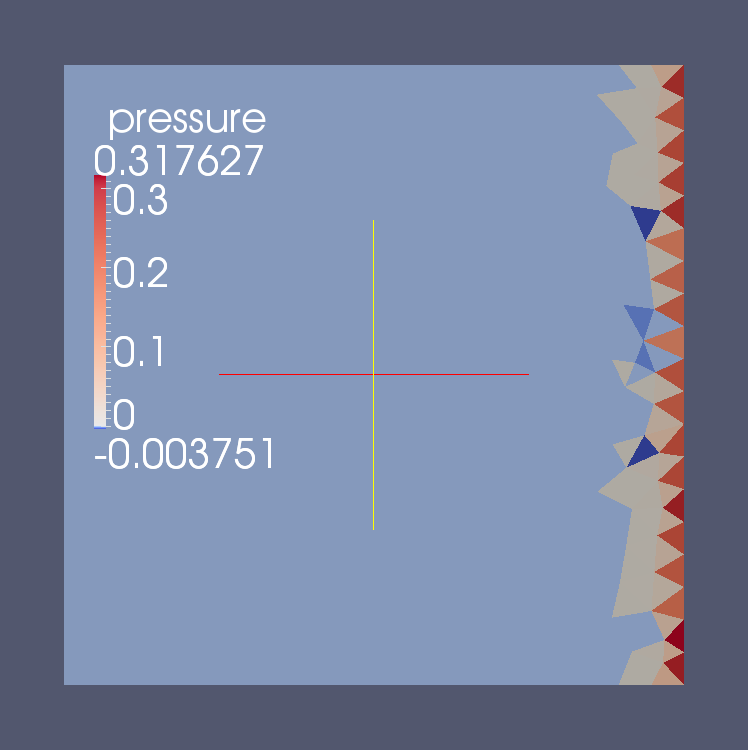
\includegraphics[width=0.4\textwidth]{MH.png}
       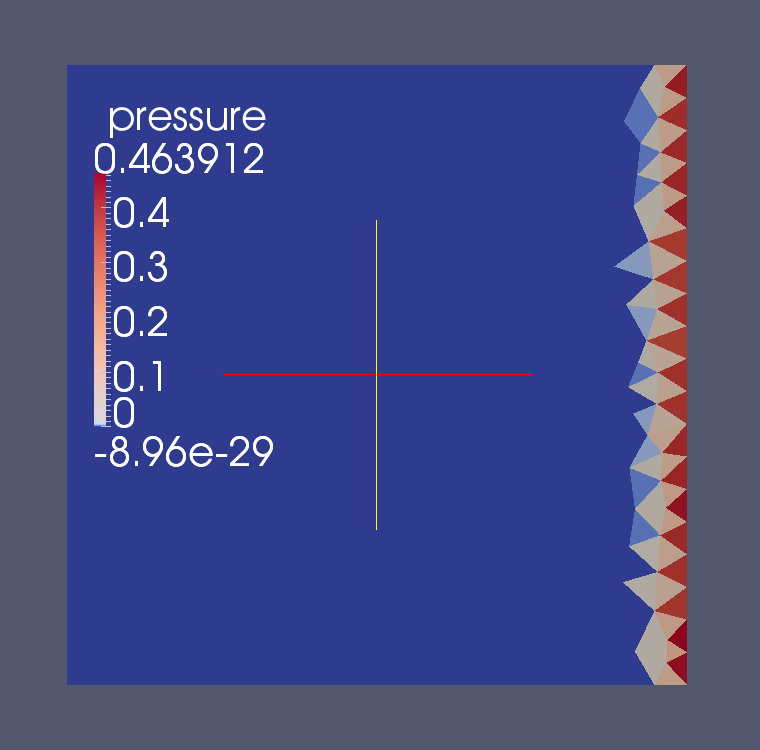
\includegraphics[width=0.405\textwidth]{LMH.png}        
    \end{center}
    \caption{Porovnání MH schématu (vlevo) a LMH schématu (vpravo), 
$\tau=10^{-4}$.}
    \label{fig:LMH}
\end{figure}





\subsection{Lineární řešič BDDCML}
\input bddcml



\section{Uživatelské rozhraní}
\subsection{Vstupní sooubor s hierarchickým formátem}
Až do verze 1.6.7 byl hlavní vstupní soubor ve formátu \verb'INI', 
ten obsahoval odkazy na další soubory se vstupními daty. Formát těchto souborů 
nebyl nijak sjednocen a pro každý soubor musela existovat samostatná čtecí 
funkce. Dokumentace těchto souborů byla neúplná.

V rámci projektu bylo navrženo nové vstupní rozhraní s následujícími 
vlastnostmi.
\begin{itemize}
\item Rozhraní umožňuje deklarovat hierarchickou strukturu vstupů 
přímo ve zdrojovém kódu a to nezávisle na konkrétním formátu vstupního souboru.
%
\item V rámci deklarace je možné vstupy dokumentovat a tuto dokumentaci je 
možné vypsat uživateli nebo vygenerovat technickou dokumentaci pomocí 
typografického systému \LaTeX.
%
\item Rozhraní implementuje čtení vstupních dat z 
vhodných hierarchických vstupních formátu (aktuálně podporován formát JSON s 
drobnými rozšířeními). Během čtení je prováděna kontrola vstupních dat vůči 
deklarované struktuře.
%
\item Rozhraní poskytuje jednotný přístup k načteným datům na straně programu. 
\end{itemize}

V průběhu roku 2012 bylo toto vstupní rozhraní implementováno. Struktura 
vstupních dat je popsána pomocí tříd (ve jmenném prostoru \verb'Inut::Type') 
pro základní typy dat: \verb'String', \verb'Bool', \verb'Integer', 
\verb'Double', \verb'FileName' a \verb'Selection' (obdoba typu enum z jazyka 
C). Objekty třídy \verb'Array' definují složený datový typ, seznam dat 
stejného typu, ke kterým se přistupuje pomocí pořadí. Objekty třídy 
\verb'Record' definují složený datový typ, kde se k jednotlivým datů přistupuje 
přes pojmenované klíče, přičemž tato data mohou být různého typu. Objekty třídy 
\verb'AbstractRecord' umožňují jednoduchou dědičnost a zejména polymorfismus. 
Typ \verb'Record' může být definován jako potomek nějakého typu 
\verb'AbstractRecord'. Polymorfismus dovoluje definovat pole 
\verb'Array' sestávající z dat nějakého \verb'AbstractRecord' typu $X$.
Na vstupu pak lze do pole ukládat data libovolných 
\verb'Record' typu $Y$, pokud $Y$ je potomkem $X$. Vstup pro typy 
\verb'AbstractRecord' musí obsahovat speciální klíč \verb'TYPE', který 
specifikuje jméno \verb'Record' typu (potomka), který se na vstupu vyskytuje. 
V programu je tak možno vytvořit instanci příslušné třídy.
Takto je možno deklarovat velice obecnou hierarchickou strukturu vstupních dat 
se zahrnutím dokumentace a implicitních hodnot.

Byly implementovány třídy pro výstup deklarované hierarchie v několika 
formátech. Zadáním vhodných argumentů programu Flow123d na příkazové řádce
lze vypsat hierarchii vstupu v několika formátech:
\begin{itemize}
 \item Textový formát. (parametr \verb'--full_doc') Vypíše úplný popis 
hierarchie v textovém formátu či
 \item LaTeX formát. (parametr \verb'--latex_doc') Vygeneruje úplný popis 
hierarchie v LaTeX formátu. Spolu se sadou speciálních maker je možné 
vygenerování PDF s technickou dokumentací a její propojení s ručně psanou částí 
pomocí hyperlinků. 
 \item JSON strojově čitelný formát. (parametr \verb'--JSON_machine') Vygeneruje 
úplný popis hierarchie ve formátu JSON, který je vhodný pro strojové 
zpracování. Do budoucna umožní například tvorbu grafického nástroje pro 
přípravu vstupních dat.
\end{itemize}


Dále byla implementována čtečka datového formátu JSON. Pro lepší srozumitelnost 
vstupních souborů byla zahrnuta možnost vkládání komentářů (není součást 
standardu JSON, ale součást jazyka JavaScript, jehož je JSON součástí). 
Pro lepší čitelnost vstupních souborů dovoluje čtečka vynechání uvozovek u 
jmen klíčů a použití rovnítka pro přiřazení hodnoty (místo dvojtečky).
Čtečka provádí kontrolu vstupu oproti jeho deklaraci a jednotným způsobem hlásí 
chyby na vstupu včetně jejich logické pozice ve vstupním souboru. Načtená data 
jsou ukládána do jednoduché stromové struktury, odkud jsou přístupná 
prostřednictvím přístupových tříd \verb'Record', \verb'AbstractRecord' a 
\verb'Array' (ze jmenného prostoru \verb'Input'), které umožňují čtení pomocí 
klíče (třída \verb'Record') respektive pomocí iterátoru (třída \verb'Array').

Vstupní rozhraní plně nahradilo dřívější hlavní \verb'INI' soubor a umožnilo 
lépe strukturovat a dále rozšiřovat strukturu vstupních dat. Pro snadnější 
přechod na nový formát vstupních dat byl vytvořen jednoduchý konvertor 
\verb'INI' souboru do formátu JSON s příslušnou novou strukturou.  

\subsection{Zadávání časoprostorových fyzikálních polí}
S využitím nového vstupního rozhraní byla vytvořena hierarchie tříd (Field) pro 
jednotný vstup časoprostorových skalárních, vektorových či 
tenzorových polí. Tento přístup nahradil všechny další vstupní soubory 
s výjimkou souborů s výpočetní sítí. Další výhodou je možnost zadávat data 
nezávisle na konkrétní síti, ale pouze v  návaznosti na její geometrii danou 
soustavou regionů.

Naprostou většinu parametrů rovnic lze chápat jako funkce času a polohy ve 
výpočetní oblasti nebo její hranici (okrajové podmínky).  Třída 
\verb'Field', respektive šablona parametrizovaná typem 
závislé hodnoty (diskrétní, skalár, vektor, tenzor), reprezentuje 
takovéto funkce. Třída zejména implementuje  metodu pro výpočet 
závislé hodnoty pro daný čas a bod ve výpočetní oblasti.
Z důvodů efektivní implementace se metodě předává jako parametr i 
element, na kterém bod leží. Množina elementů tvořících jednu logickou 
oblast (např. jeden materiál) se nazývá {\emph region}. Třída \verb'Field' 
obsahuje tabulku, která každému regionu přiřazuje instanci třídy (respektive 
šablony) \verb'FieldBase'. Potomci této třídy implementují vlastní výpočet 
závislé hodnoty pro konkrétní region. Volbou potomka (pomocí klíče 
\verb'TYPE') může uživatel zvolit algoritmus použitý pro výpočet závislé 
hodnoty. V současné době jsou implementovány třídy:
\begin{itemize}
 \item {\tt FieldConstant} 
 --- zadání konstantní hodnoty na regionu.
 \item {\tt FieldFormula} 
 --- zaání funkce pomocí vzorce obsahujícího proměnné 
 $t$, $x$, $y$,$z$.
 \item {\tt FieldPython} 
 --- umožňuje výpočet hodnot pomocí funkce v jazyce Python.
 \item {\tt FieldElementwise} 
 --- diskrétní funkce po částech konstantní na elementech sítě. Hodnoty 
ve formátu GMSH dané ve zvláštním souboru. Vyžaduje data zadaná na stejné síti 
jako je síť výpočetní. 

 \item {\tt FieldInterpolated}
 --- diskrétní funkce po částech konstantní na elementech sítě. Hodnoty 
jsou interpolovány ze sítě a dat ve formátu GMSH dané ve zvláštním souboru.
\end{itemize}

Koncept {\emph Fields} byl natolik úspěšný, že byl dále rozšířen i pro 
předávání vypočtených fyzikálních polí do výstupního rozhraní a mezi 
rovnicemi.

{\bf Interpolace mezi sítěmi.}
Aktuálně je implementována interpolace po částech konstantních dat z 3D sítě na 
data konstantní na 2D a 1D elementech. Interpolovaná hodnota na elementu $X$ je 
vypočtena jako vážený průměr hodnot na elementech mající s $X$ neprázdný 
průnik. Váhy jsou dány velikostí průniku.
Pro efektivní výpočet je třeba k danému 
elementu $X$ cílové sítě najít seznam elementů zdrojové sítě, které mají s $X$ 
neprázdný průnik a to maximálně se složitostí $O(log N)$ vzhledem k velikosti 
zdrojové sítě. Toho je dosaženo vytvořením vyhledávacího stromu nad elementy 
zdrojové sítě, konkrétně je použita metoda \uv{Bounding interval hierarchy}
(BIH). 
Vyhledávací strom BIH pro zadaný element vytvoří obalový box a vrátí seznam 
elementů jejichž obalové boxy s ním mají neprázdný průnik. Pro každý takový 
element podezřelý z průniku, je třeba nalézt skutečný průnik se vstupním 
elementem. Toto je zatím implementováno jen pro dvojice 3D-2D a 3D-1D elementů. 
Rozpracovaný je výpočet průniků pro další kombinace dimenzí a algoritmy 
pro hledání všech průniků v lineárním čase.

\subsection{Systém chybových hlášení}
Pro snadné používání programu je důležité dostatečně podrobné 
reportování chyb. V případě chyby by měl uživatel dostat relevantní 
informace o příčinách jejího vzniku. 
Až do verze 1.6.7 byly uživatelské i programové chyby vypisovány přímo v místě 
detekce chyby, kde ovšem často nejsou k dispozici všechny potřebné informace. 
Při vývoji vstupního rozhraní byl pro reportování chyb použit systém výjimek, 
který umožňuje zachytit výjimku ve vyšší vrstvě a přidat do ní dodatečné 
informace. Mechanismus výjimek jazyka C++ zároveň zajistí zavolání všech 
destruktorů a kontrolované ukončení programu.
Nový systém výjimek byl dále použit i v dalších částech 
programu a byly do něj zapouzdřeny i původní funkce pro vypisování chybových 
zpráv. 

\subsection{Výstupní rozhraní}
Před započetím projektu umožňoval Flow123d výstup pouze několika veličin do 
formátu GMSH. Jedná se sice o otevřený datový formát s jednoduchou strukturou, 
ale k vizualizaci a postprocesingu dat je možné použít pouze program GMSH, 
který je však primárně určen k přípravě výpočetních sítí. V rámci projektu byla 
přidána podpora pro výstup do formátu VTK, který je podporován většinou 
vizualizačních programů. Dále bylo implementováno výstupní rozhraní, které 
umožňuje výstup libovolného pole \verb'Field'. Uživatel tak může vybrat pro 
výstup jak vstupní tak vypočtená pole, případně jejich částečně zpracované 
varianty. Výstup je podporován jak do GMSH tak do VTK formátů a to pomocí třech 
různých diskretizací: data konstantní na elementech, lineární funkce na 
elementech dané hodnotami v uzlech sítě, lineární funkce na elementech 
nespojité přes hranice elementů. První varianta je přirozená pro metodu 
konečných objemů, druhé pro spojitou Galerkinovu  metodu prvního řádu a 
třetí varianta je přirozená pro nespojitou Galerkinovu metodu prvního 
řádu. Všechny varianty umožňují výstup skalárních, vektorových, i tenzorových 
dat.

\section{Kvalita kódu}

Vzhledem ke stále intenzivnějšímu vývoji a rozšiřování vývojového týmu jsme se 
rozhodli přejít na nový systém pro správu verzí (git) a nový hosting centrálního 
repozitáře (github). Tyto nástroje velmi zefektivňují týmovou spolupráci a 
organizaci vývoje. Prezentace projektu na serveru github navíc přispívá k jeho 
zviditelnění a umožňuje jednodušší spolupráci s externími vývojáři. Se změnou 
verzovacího nástroje jsme museli změnit software pro průběžnou integraci (CI) a 
testování. V současnosti používáme volně dostupný software Jenkins. Byl také 
zprovozněn nový testovací a sestavovací server jak pro systém Linux tak pro 
Windows. V současnosti tak máme k dispozici každodenní instalační balíčky pro 
Linux i Windows sestavené z aktuálního stavu vývojové větve.  Tyto poměrně 
zásadní změny si vyžádaly poměrně dost času na zvládnutí nových nástrojů a 
zaškolení týmu, výsledkem však je  infrastruktura, která nám v následujících 
letech umožní efektivně produkovat výkonný a spolehlivý software.


\begin{thebibliography}{99}

\bibitem{ern2010guaranteed}
A. Ern, A.F. Stephansen, M. Vohral{\'\i}k.
Guaranteed and robust discontinuous Galerkin a posteriori error estimates for convection--diffusion--reaction problems,
\emph{Journal of computational and applied mathematics}, 234(1):114--130, 2010.


\bibitem{ern_stephansen_zunino}
A. Ern, A.F. Stephansen, P. Zunino.
A discontinuous {G}alerkin method with weighted averages for advection--diffusion equations with locally small and anisotropic diffusivity,
\emph{IMA Journal of Numerical Analysis}, 29(2):235--256, 2009.


\bibitem{younes_2006}
A. Younes, P. Ackerer, F. Lehmann.
A new mass lumping scheme for the mixed hybrid finite element method,
\emph{Int. J. Numer. Meth. Engng}, 67:89–107, 2006.


\bibitem{martin_modeling_2005}
V. Martin, J. Jaffr{\'e}, J.E. Roberts.
Modeling Fractures and Barriers as Interfaces for Flow in Porous Media,
\emph{{SIAM} Journal on Scientific Computing}, 26(5):1667--1691, 2005.


\bibitem{millington_quirk}
R.J. Millington, J.P. Quirk.
Permeability of porous solids, 
\emph{Transactions of the Faraday Society}, 57:1200--1207, 1961.


\bibitem{SistekBDDC}
J. Šístek, J. Březina, B. Sousedík : BDDC for Mixed-Hybrid 
Formulation of Flow in Porous Media with Combined Mesh Dimensions, Numer. Linear 
Algebra Appl. (submitted)
\end{thebibliography}




\end{document}